\documentclass{article}

% if you need to pass options to natbib, use, e.g.:
% \PassOptionsToPackage{numbers, compress}{natbib}
% before loading nips_2018

% ready for submission
\PassOptionsToPackage{numbers}{natbib}
\usepackage[final]{../common/nips_2018}

% to compile a preprint version, e.g., for submission to arXiv, add
% add the [preprint] option:
% \usepackage[preprint]{nips_2018}

% to compile a camera-ready version, add the [final] option, e.g.:
% \usepackage[final]{nips_2018}

% to avoid loading the natbib package, add option nonatbib:
% \usepackage[nonatbib]{nips_2018}

\usepackage[utf8]{inputenc} % allow utf-8 input
\usepackage[T1]{fontenc}    % use 8-bit T1 fonts
\usepackage{hyperref}       % hyperlinks
\usepackage{url}            % simple URL typesetting
\usepackage{booktabs}       % professional-quality tables
\usepackage{amsfonts}       % blackboard math symbols
\usepackage{nicefrac}       % compact symbols for 1/2, etc.
\usepackage{microtype}      % microtypography
\usepackage{graphicx}

\title{CS224n Project Proposal}

% The \author macro works with any number of authors. There are two
% commands used to separate the names and addresses of multiple
% authors: \And and \AND.
%
% Using \And between authors leaves it to LaTeX to determine where to
% break the lines. Using \AND forces a line break at that point. So,
% if LaTeX puts 3 of 4 authors names on the first line, and the last
% on the second line, try using \AND instead of \And before the third
% author name.

\author{
  Luis A. Perez \thanks{} \\
  Department of Computer Science\\
  Stanford Univeristy\\
  Stanford, CA 94305 \\
  \texttt{luis0@stanford.edu} \\
  %% examples of more authors
  %% \And
  %% Coauthor \\
  %% Affiliation \\
  %% Address \\
  %% \texttt{email} \\
  %% \AND
  %% Coauthor \\
  %% Affiliation \\
  %% Address \\
  %% \texttt{email} \\
  %% \And
  %% Coauthor \\
  %% Affiliation \\
  %% Address \\
  %% \texttt{email} \\
  %% \And
  %% Coauthor \\
  %% Affiliation \\
  %% Address \\
  %% \texttt{email} \\
}

\begin{document}
% \nipsfinalcopy is no longer used

\maketitle

\begin{abstract}
  We propose working on the default final project, in the PCE-division, in an attempt to improve currint SOTA results in the SQuAD NLP task. In particular, we propose experimenting with several extensions of BERT \cite{BERT} (such as a few of those proposed in the handout), performing thorough error analysis, and finally creating an ensemble from these extensions. 
\end{abstract}

\section{Research Paper Summary}
We summarize the paper by Jacob Devlin, Ming-Wei Chang, Kenton Lee, and Kristina Toutanova from the Google AI Language Lab titled ``BERT: Pre-training of Deep Bidirectional Transformers for Language Understanding'' \cite{BERT}. The paper is chosen since it is currently the foundation for the vast majority of high-performing models in the SQuAD 2.0 leaderboard. See Table \ref{table:top_10_squad} for a list of the top-ten models, and note that all of these models make use of the BERT architecture + weights as a foundation for their work. 

\subsection{Background and Context}
The authors of this paper set-out on the task of creating a pre-trained, non-task-specific language model with the end-goal of using this model to further the SOTA results in task-specific metrics, such as GLUE and SQuAD v1.1. Their work can be considered an extension of ELMO \cite{ELMO}, which introduced \textit{deep contextualized} word representations, rather than static, fixed-size word representations used previously, such as those in word2vec. These representations can better model complex characteristics of word use and how these uses vary across lingustic contexts. BERT follows the same core idea as ELMO -- extending the embeddings for a word be using the context in which it appears to modify them. The major contribution of the BERT \cite{BERT} paper and its authors is to take this same idea, but rather than using traditional encoder-decoder architectures based on RNNs, they instead make use of the Transformer architecture. 

With these pre-trained language representations, task-specific models can be utilized downstream through two main strategies (1) feature-based and (2) fine-tuning. The former essentially includes the pre-trained language representations along with additional features, to train a new model, while the latter simply fine-tunes the pre-trained parameters (without introducing too many new parameters).

Transformer had already demonstrated their utility and power in task-specific contexts, such as SQuAD and others. As such, using them for the task of creating context-aware word-embeddings was not far-fatched.

\subsection{Problem and Proposed Solution}
The paper \cite{BERT} is specifically trying to solve the problem of learning and improved language model for use in word-representations. The proposed solution is to use a large corpus of text and a bi-directional transformer-centric architecture which leads to much improved word-embeddings.

The authors address issues with previous models (such as unidirectionality) by proposing two new pre-training objectives:
\begin{itemize}
    \item The ``masked language model''. 
    \item The ``next sentence prediction''.
\end{itemize}

The major contribution, then, from the BERT paper is (1) the introduction of pre-training objectives independent of final objectives, (2) utilization of bi-directional models to take full advantage of the language model, and (3) a pre-trained model which achieves SOTA results across multiple, distinct NLP tasks after fine-tuning, with a single additional layer. The key achievement is a 4.4\% to 6.7\% average accuracy improvement over previous SOTA models in the GLUE benchmarks. The full results (for all benchmarks) are reproduced in Table \ref{fig:bert_glue_results} from the paper. The best performing BERT system also outperforms the top leaderboard system by +1.5 F1 in ensembling and +1.3 F1 on a single system. For more details, see Table \ref{fig:bert_squad_results}. 

\subsection{The BERT Model}
BERT's model architecture is simply a multi-layer bidrectional Transformer encoder based on the original implementation by Vaswani et al \cite{AttentionIsAllYouNeed} and as detailed in Figure \ref{fig:bert_architecture_comparison}. Transformers help reduce the number of operations required to learn long-distance dependencies to a constant number (at the cost of resolution). They make use of stacked self-attention and point-wise, FC layers for the encoder and decoder, as can be seen in Figure \ref{fig:transformers}. A detailed discussion of this architecture (by annotating the paper that introduced it), can be found \href{http://nlp.seas.harvard.edu/2018/04/03/attention.html}{here}, and is also covered in class. As such, we defer any further details.

\subsection{The BERT Pre-training Tasks}
For all of the tasks described below, a concatenation of the BooksCorpus (800M words) and English Wikipedia (2,500M words) is used (only text, no lists/tables/headers).

\subsubsection{Masked Language Model MLM}
In this context, the goal for the model is not task-specific (ie, such as SQuAD), but rather, input data has tokens randomly masked (removed), and the goal is to generate a model that, given this incomplete data, can correctly identify the original vocabulary id. One key aspect of this task is that the model has access to both previous words \textbf{and} future words. Further, it is different from auto-regressive models in that only the hidden state for the masked-word is used to compute the softmax probabilities over the vocabulary.

To soften the mismatch between pre-training on this task and fine-tuning on future tasks, the [MASK] token is not actually always used. As per the paper, it is used only 80\% of the time, while 10\% of the time the token is not masked at all, and the remaining times it is replaced by a random word.

\subsubsection{Next Sentence Prediction}
Interestingly enough, this task is utilized as an attempt to improve the performance of BERT on future QA and NLI tasks. In fact, this contradicts the fact that BERT is simply a language model without specific characteristics to the tasks it eventually achieves SOTA results in. 

The task consists of pre-training a binarized \textit{next sentence prediction} task on a large corpus. This task also helps explain the input representation chosen for the BERT model, which consists of 3 distinct pieces: (1) token embeddings, from WordPiece embeddings, (2) Segment Embeddings (only two segments are used, A and B, which assists on using BERT for the next sentence prediction task), and (3) position embeddings (BERT only supports sequences up to 512 in length).

\subsection{BERT Fine-Tuning}
A key insight of the paper is introducting the ability to use a single, pre-trainined system which can then be fine-tuned for specific tasks. Here, we summarlize the modifcations which were made in order to handle each of the NLP tasks which the system tackled. In broad-strokes, there are essentially two types of tasks which the system handles: (1) sequence classification and (2) question-answer pairs. 

\subsubsection{Sequence Classification}
These are mostly from the GLUE benchmark, and consists of tasks where a sequence is fed into the model and a classification needs to occur (across C classes). The amazing thing about BERT is that it achieves state of the art results in these tasks only through fine-tuning. Specifically, the model takes as input a special [CLS] token as the first token (this was also done during pre-training), and the hidden state output from the transformer model (BERT) corresponding to this input token, is take as the hidden state input for a linear classifier. 

That is to say, the fine-tuning consists simply of learning a $W \in \mathbb{R}^{K \times H}$, where $K$ is the number of labels and $H$ is the dimension of the hidden state, $C$, output from the transformer model (BERT). These new parameters (as well as the BERT parameters) can then be trained on this task.

\subsubsection{Question and Answers}
The BERT paper focuses on the SQuAD task, a collection of 100k corwdsourced question/answer pairs. For this system, we take advantage of the input representation used by BERT. The question tokens correspond to the sentence 1 encoding, and the paragraph to the sentence 2 encoding. Then each output transform state, $T_i$ is dot-produced with two new parameter vectors, $S$ and $E$ for start and end. The a straightforward softmax is taken from this dot-product for all $i$, to determine the start and end of the corresponding answer in the text. Similar modifications are used for other tasks, which are detailed further in the paper. 

\subsection{Concluding Remarks}
Overall, the paper presents an attention-based mechanism for pre-training on a large-corpus of data. Furthermore, due to the architectural choices and the input representations, this pre-trained model called BERT can be fine-tuned, with the addition of a few final layers, to achieve SOTA performance across many tasks. 

\section{Project Description}
\subsection{Goals}
The primary goal of the project is to explore alternative, more complex architectures for fine-tuning the BERT model, and explore whether or note these modifications provide meaninful improvements.

In particular, we find the approach in \cite{BERT} for classification tasks to be severely limiting, as it attempts to condence the entirety of the contextual information into a single hidden-state. We propose exploring a few natural extension to this approach to determine if it's possible to achieve better results with a more complex fine-tuning architecture. We believe doing this will provide valuable theoretical insight as to the power of BERT, as well as provice practical direction and guidance for future systems seeking to perform task-specific objectives through fine-tuning.

\begin{itemize}
    \item Do we need fine-tuning layer? Here, we propose an extreme, where we actually seek to analyze and understand the results of using BERT with no additional fine-tuning layers.
    \item What if it were deeper? Here, we propose an extension, where additional intermediate convolutional layers are used rather than a single FC layer on the classification hidden state. We suspect that this will lead to some improved performance on the fine-tuned tasks, since the model will have increased flexibility and capacity.
    \item Can we make use of the other transformer hidden states? Our hypothesis is that currently fine-tuned BERT models are bottlenecked by the single hidden-state. Instead, we propose making use of all of the transformer hidden states for classification
    \item Both of the above approaches are also equally applicable to the other metrics used in the BERT paper.
\end{itemize} 

Our primary goal is to explore these alternatives, analyze the results, and make an educated attempt at improving current SOTA systems.

As an extension goal, we'd like to approach the task of answer generation for the SQuAD datasets. This task is still not very well-defined, but the overall goal would be to, rather than pin-point to the part of the text where the answer to the question exists, instead create a generative model that can propose multiple answer and generate the output sequence itself. This can be an extension of the BERT model where the transformer states are attended to all out once and fed as input.

The metric would be to use BLEU against the correctly extracted sentence text. In a failure mode, the model would actually learn simply to find the answer text and generate it. However, we'd like to avoid this happening. 

\subsection{NLP Tasks}
The NLP task is the same as those addressed in \cite{BERT}, with an emphasis on SQuAD V2.0 as this is the default project. We'd like to achieve good performance on this new task, by making use of the above proposed modifications.

\subsection{Data}
The dataset is already pre-specified by the default final project handout. However, for our own edification and for our stretch goals, we plan to make use of the GLUE datasets and mini-tasks to more accurately evaluate the validity of our results across multiple NLP tasks. 

\subsection{Varients}
As discussed in the goal section, we propose making a few modifications to the fine-tuning aspect of BERT in order to make better use of the information available.

In particular, for classification tasks, we suspect that the single hidden state used is actually a bottleneck to be overcome. We propose overcoming this bottleneck through multiple possible mechanisms such as (1) an attention later to combine all of the final BERT outputs into a classification hidden state or (2) a RNN which takes the hidden outputs as well as the classificatio hidden state to generate the final classification scores (3) more deep/complex architectures, such as a residual block using 1D convolutions.

Furthermore, some of the above described varients can also be utilized to hopefully improve on the SQuAD v2.0 task. 

\subsection{Baselines}
The baseline model for SQuAD V2.0 will be existing SOTA systems. The baseline model for the GLUE metrics will be the original results reported by the BERT \cite{BERT} paper, as we will be doing an extension attempting to understanding the utility and extensiveness of fine-tuning.

\subsection{Result Evaluation}
As discussed above, SQuAD v2.0 will be used as the default, automatic evaluation metric for all of the modifications proposed above (for the SQuAD task). For the classification tasks, we will use the GLUE to evaluate our model's performance. 

\section{Appendix}

\begin{table}[!ht]
\centering
\begin{tabular}{l|l|l|l}
Model/Method                   & Category       & EM     & F1     \\ \hline
BERT + MMFT+ ADA               & BERT Ensemble  & 85.082 & 87.615 \\
BERT + Synthetic Self-Training & BERT Ensemble  & 84.292 & 86.967 \\
BERT finetune baseline         & BERT Ensemble  & 83.536 & 86.096 \\
Lunet + Verifier + BERT        & BERT Ensemble  & 83.469 & 86.043 \\
PAML + BERT                    & BERT Ensemble  & 83.467 & 86.035 \\
Lunet + Verifier + BERT        & BERT Extension & 82.995 & 86.035 \\
BERT + MMFT + ADA              & BERT Extension & 83.040 & 85.892 \\
BERT + Synthetic Self-Training & BERT Extension & 82.975 & 85.810 \\
PAML + BERT                    & BERT Extension & 82.577 & 85.810
\end{tabular}
\caption{Table with Top 10 models/methods on SQuAD 2.0 as of 2/12/2019. See \href{https://rajpurkar.github.io/SQuAD-explorer/}{SQuAD Leaderboard} for more details.}
\label{table:top_10_squad}
\end{table}

\begin{figure}[!ht]
\centering
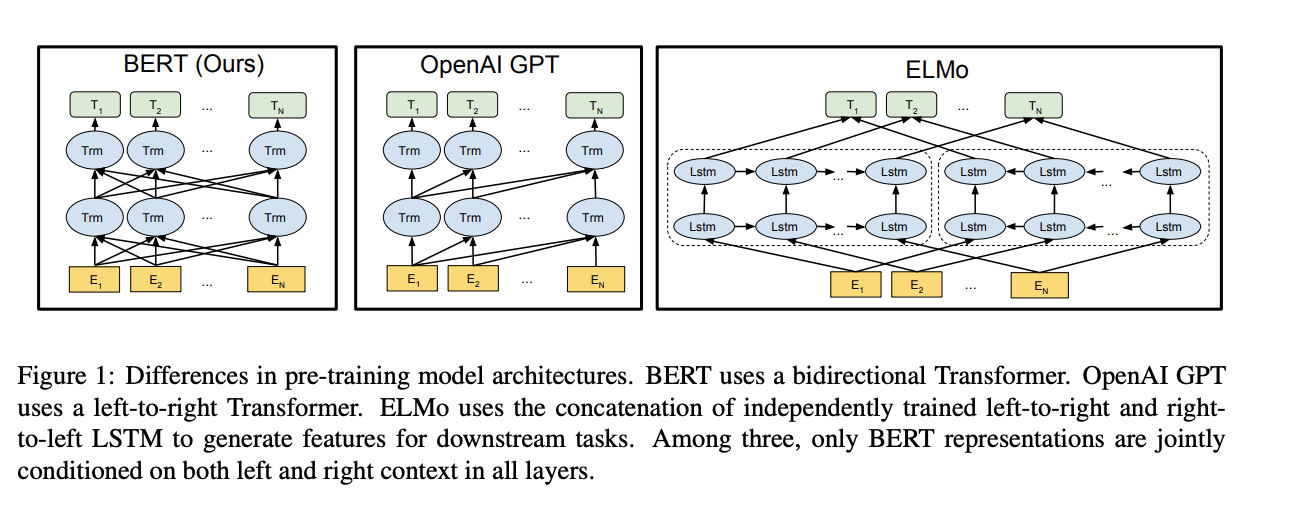
\includegraphics[scale=0.7]{../figures/BERT_architecture_comparsion}
\label{fig:bert_architecture_comparison}
\end{figure}


\begin{figure}[!ht]
\centering
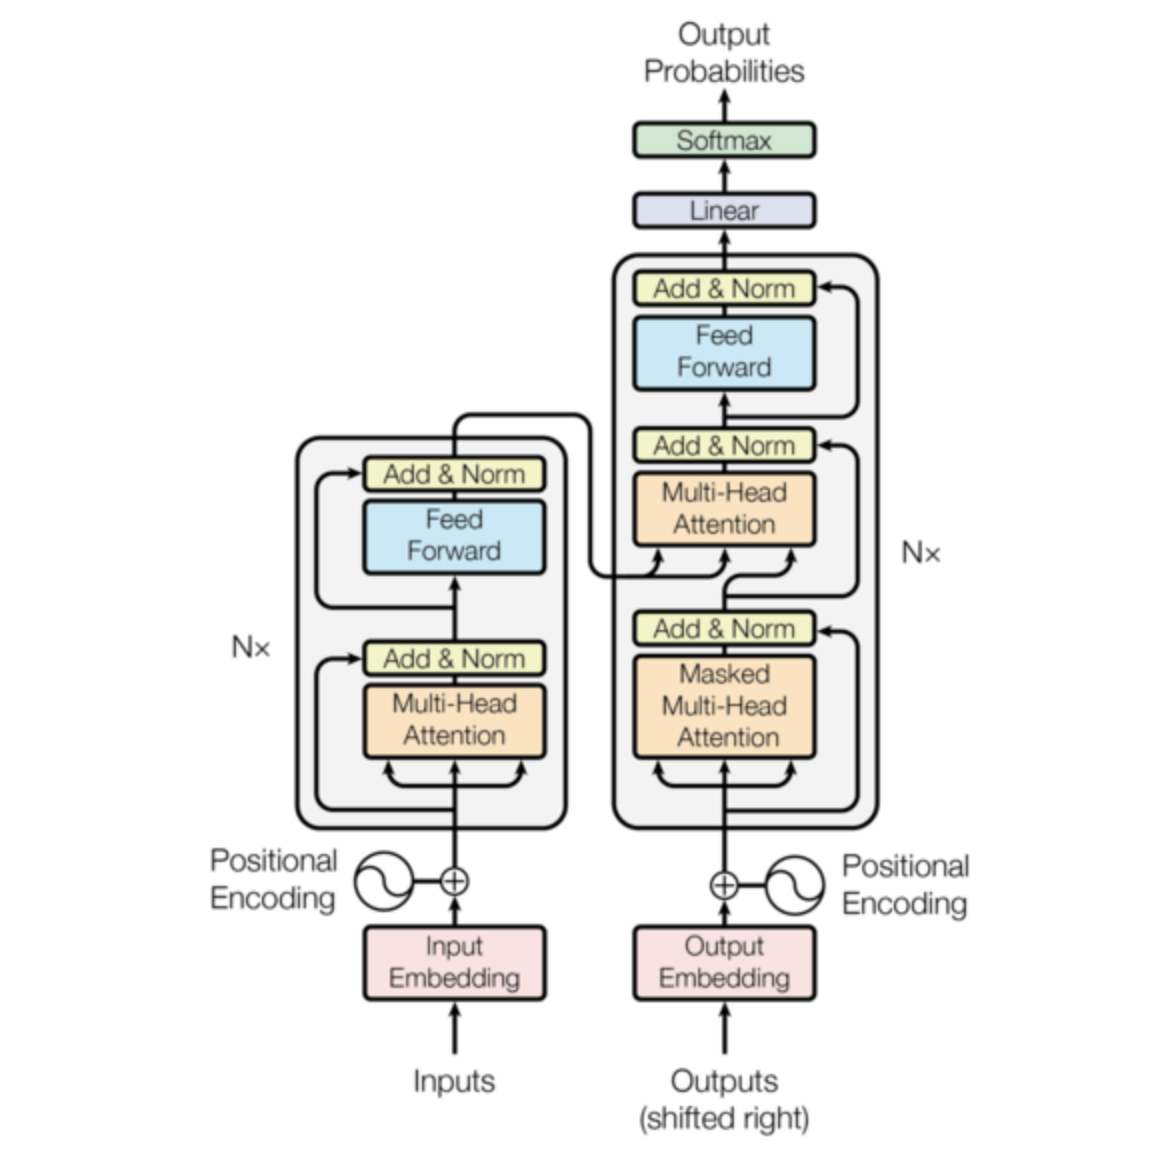
\includegraphics[scale=0.7]{../figures/Transformers}
\label{fig:transformers}
\end{figure}

\begin{figure}[!ht]
\centering
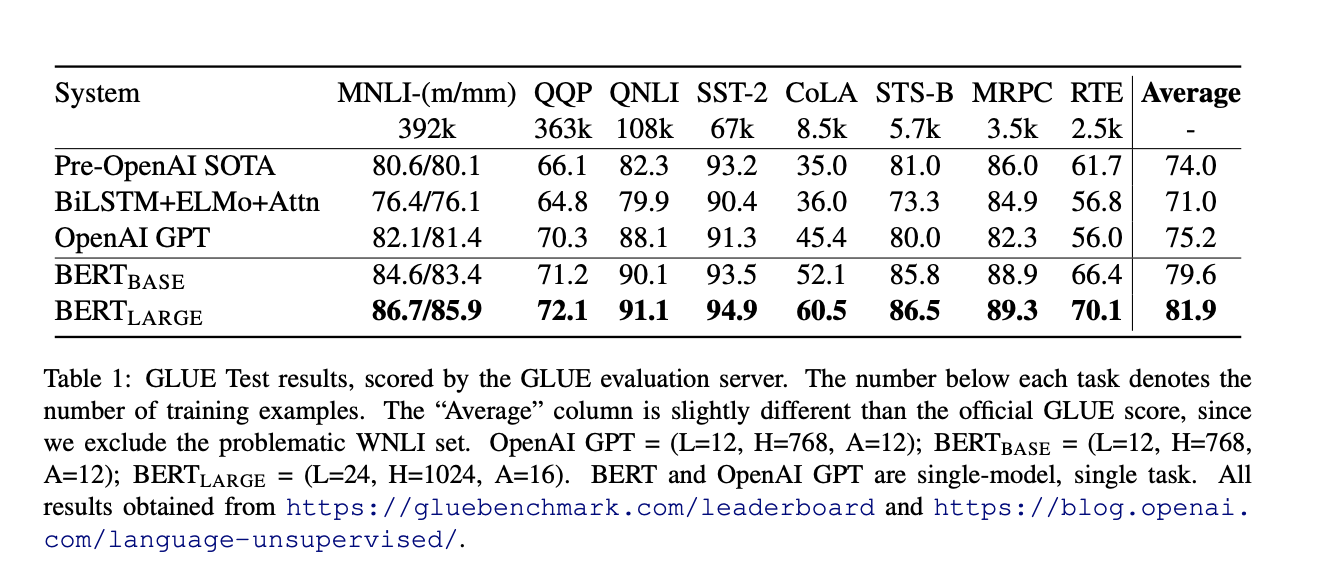
\includegraphics[scale=0.7]{../figures/BERT_GLUE_results}
\label{fig:bert_glue_results}
\end{figure}

\begin{figure}[!ht]
\centering
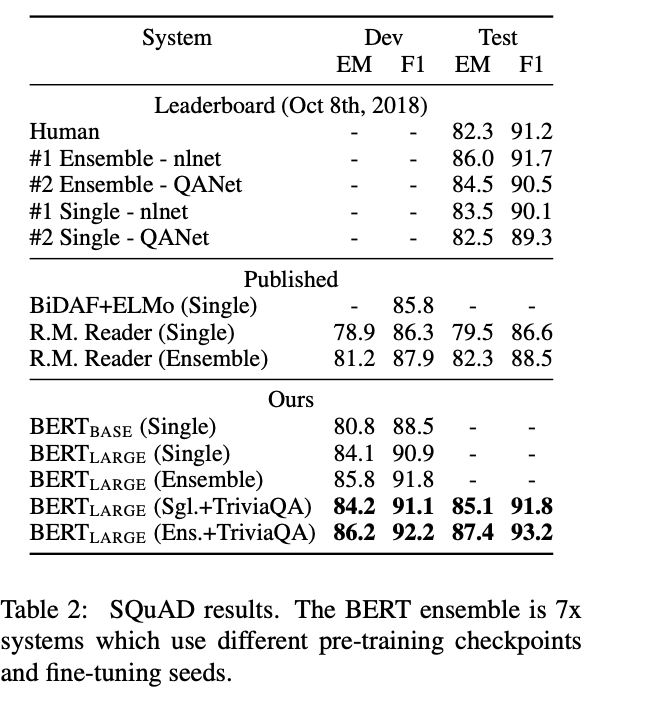
\includegraphics[scale=0.7]{../figures/BERT_SQuAD_results}
\label{fig:bert_squad_results}
\end{figure}

\section*{References}

{\small
\bibliographystyle{../common/ieee}
\bibliography{../common/egbib}
}

\end{document}
